
%%%%%%%%%%%%%%%%%%%%%%% file typeinst.tex %%%%%%%%%%%%%%%%%%%%%%%%%
%
% This is the LaTeX source for the instructions to authors using
% the LaTeX document class 'llncs.cls' for contributions to
% the Lecture Notes in Computer Sciences series.
% http://www.springer.com/lncs       Springer Heidelberg 2006/05/04
%
% It may be used as a template for your own input - copy it
% to a new file with a new name and use it as the basis
% for your article.
%
% NB: the document class 'llncs' has its own and detailed documentation, see
% ftp://ftp.springer.de/data/pubftp/pub/tex/latex/llncs/latex2e/llncsdoc.pdf
%
%%%%%%%%%%%%%%%%%%%%%%%%%%%%%%%%%%%%%%%%%%%%%%%%%%%%%%%%%%%%%%%%%%%


\documentclass[runningheads,a4paper]{llncs}

\usepackage{amssymb}
\setcounter{tocdepth}{3}
\usepackage{graphicx}
%\usepackage{hyphenat} see
%http://www.ctan.org/tex-archive/macros/latex/contrib/hyphenat - would
%be good to enable this to prevent hyphenation of OWL MS statements.
%Or find alternative

\usepackage{url}
%\urldef{\mailsa}\path|davidos@ebi.ac.uk|

\newcommand{\keywords}[1]{\par\addvspace\baselineskip
\noindent\keywordname\enspace\ignorespaces#1}

\def\correspondingauthor{$^*$}
\def\@corresponding{\footnotesize\correspondingauthor Corresponding author} 


\begin{document}

\mainmatter  % start of an individual contribution

% first the title is needed
\title{Virtual Fly Brain - Using OWL to support the mapping and
  genetic dissection of the \textit{Drosophila} brain.}

% a short form should be given in case it is too long for the running head
\titlerunning{Virtual Fly Brain - using OWL to support Drosophila neurobiology}

% the name(s) of the author(s) follow(s) next
%
% NB: Chinese authors should write their first names(s) in front of
% their surnames. This ensures that the names appear correctly in
% the running heads and the author index.
%
\author{David Osumi-Sutherland$^1*$, Marta Costa$^2$, Robert
  Court$^3$, Cahir J. O'Kane$^2$}

%
\authorrunning{Virtual Fly Brain - using OWL to support Drosophila neurobiology}
% (feature abused for this document to repeat the title also on left hand pages)

% the affiliations are given next; don't give your e-mail address
% unless you accept that it will be published
\institute{$^1$ European Bioinformatics Institute (EMBL-EBI)
European Molecular Biology Laboratory
Hinxton, Cams, UK\\
$^2$Department of Genetics, University of Cambridge, Cambridge, UK\\
$^3$School of Informatics, University of Edinburgh, Edinburgh UK}
%* corresponding author: davidos@ebi.ac.uk

% \mailsa\\  % This needs to be fixed!

%
% NB: a more complex sample for affiliations and the mapping to the
% corresponding authors can be found in the file "llncs.dem"
% (search for the string "\mainmatter" where a contribution starts).
% "llncs.dem" accompanies the document class "llncs.cls".
%

\toctitle{}
\tocauthor{}
\maketitle


\begin{abstract}
A massive effort is underway to map the structure of the \textit{Drosophila}
nervous system and to genetically dissect its function. Virtual Fly
Brain (VFB; \url{http://www.virtualflybrain.org}) is a popular, OWL-based resource
providing neuroinformatics support for this work.  It provides: curated
descriptions of brain regions and neurons; queries for neurons based
on their relationship to gross neuroanatomy; and queries for reagents
based on their expression patterns. Query results are enriched by OWL
axiomatisation allowing basic mereological reasoning.

To keep reasoning fast and scalable, VFB confines expressiveness to
the EL profile of OWL. As a result, VFB does not provide queries
involving negation, despite there being both demand and sufficient
information to support them. Recent developments in
reasoning technology may make more expressive queries practical.  Here
we present design patterns to support queries with negation that are
compatible with the mereological reasoning used in VFB.

\keywords{OWL, neurobiology, neuron, DL reasoning, negation, closure
  axioms, ontology design pattern}
\end{abstract}

\section{Introduction}


\subsection{Mapping and genetically dissecting the \textit{Drosophila}
  nervous system}


A massive effort is underway to map the neural circuitry of the
\textit{Drosophila} nervous system and to genetically dissect its
function. New microscopy and image analysis techniques are
facilitating the collection and integration of the massive 3D image
data sets required to map the structure and connectivity of the
nervous system down to the single neuron level
\cite{pmid21129968,Manton2014}. New genetic
techniques allow researchers to precisely target elements of the
neural circuitry to inhibit or activate it in order assess the effects
on nervous system function and behaviour \cite{pmid22205518}. The scale of this 
effort, and the huge volumes of data involved, mean that its success
depends on suitable informatics support. Virtual Fly Brain (VFB)
\cite{pmid22180411,pmid22402613} is an OWL-based, open source
resource dedicated to this role. Usage is growing rapidly among the community
it serves.  The site currently gets 15-20,000 page views per month.

The adult \textit{Drosophila} nervous system contains an estimated
200,000 neurons.  These can be grouped into classes that share
similar location, morphology and lineage.  As there are multiple
members of many of these classes per brain, the number of such classes
is likely to be at least an order of magnitude smaller than the number
of neurons.  Mapping the neural circuitry of \textit{Drosophila}
requires ways to track the classification of these neurons and their
properties, including their relationships to each other and to the
gross anatomy of the nervous system, musculature, sense organs and
neuro-endocrine system.  This work requires synthesis of many of
qualitative assertions from the literature and its integration with
information from bulk data sources, much of it quantitative.  OWL
is an ideal technology for building and maintaining these queryable
classifications. There will always be a need for direct mathematical
access to quantitative data.  But if suitable cutoffs can be
chosen to make qualitative assertions from quantitative data, OWL
provides a means to integrate qualitative and quantitative data into a
queryable whole.

Modulating the activity of specific neuron classes requires finding
reagents whose expression is sufficiently specific. Finding such reagents
frequently requires mining 3D image data of expression patterns.
Integrating the phenotypic results of modulating neuronal activity
into the bigger picture of nervous system function requires ways to
keep track of the phenotypes associated with modulating the neuronal
activity of connected neurons.  Annotation with OWL ontology terms -
either semi-formalised in a database or fully formalised in an OWL
knowledgebase provides a means of storing this information in
queryable form.

\subsection{Virtual Fly Brain}

\subsubsection{The Drosophila anatomy ontology.}

Virtual Fly Brain is built around the \textit{Drosophila} anatomy
ontology (DAO) \cite{Costa2013}, an OWL ontology of
\textit{Drosophila} anatomy, over 45\% of which (3875/8576 classes) is
devoted to representing neuroanatomy. The DAO is largely manually
curated from the literature and includes a large textual component in
the form of referenced synonym lists and definitions/descriptions -
making it searchable by and accessible to biologists.  These are used
to drive auto-suggestion based searching on VFB and to populate term
information pages for specific neuron classes and nervous system
regions. The DAO is also richly formalised, using 44 object properties
in \textgreater 17000 Subclassing axioms and \textgreater 2000
Equivalent Class axioms.  This axiomatisation infers almost 50\% of
\textgreater 10,000 classifications and allows a rich variety of
biologically interesting queries. In order to keep reasoning
tractable, expressiveness is kept almost entirely within the EL
profile of OWL\footnote{We stray outside the EL
  profile with inverse objectProperty declarations. To our
  knowledge, and based on extensive testing, these have no effect on classification and query
  answering with our current axiomatisation.}, allowing us to use the fast reasoner ELK \cite{kazakov2012elk}.
Classification of the ontology is complete in under 500ms.  Query
answering  time, taking advantage of incremental reasoning via ELK, is
in the 10s of ms range.

\subsubsection{Annotation queries.}

One major usage of VFB is as a means to query for expression of genes,
transgenes and phenotypes in specified anatomical classes.  These
queries use information curated from the literature and bulk data sets
by VFB and FlyBase curators using an semi-formalised tagging
system. All queries of these annotations start with a query for
subclasses, parts and overlapping cells.  The resulting list is then
used to query the FlyBase SQL database of annotations.  10's of
thousands of annotations are available from these queries.


\subsubsection{OWL queries and design patterns for neuroanatomy.}

The DAO uses an integrated set of relations and design patterns to
classify neurons according to their location, connectivity, lineage
and function \cite{pmid22180411,pmid22402613}.  The neuronal
connectivity relations (defined in detail \cite{pmid22402613})  drive the query system on VFB (see figure
\ref{fig:Query_menus_DL_images}). VFB takes advantage of term
classification in the DAO to serve only queries that are
appropriate to the term displayed. So, for example, the queries
available for neurons are different to those available for brain regions.

The typical mereological relationship between a neuron and gross
neuroanatomy is overlap:  most neurons have parts in many
parts of the brain.  In an insect brain, each neuron has a cell body
(soma) in the cortex and many have long, branching projections that extend
to multiple brain regions.  Projections bundle (fasciculate)
together to form tracts.  On exiting a tract, the projection enters a
region called neuropil where it typically branches extensively and
connects to other neuron projections via synapses.

The \textit{Drosophila} brain contains many neuron classes that can be
defined via some combination of: soma location, tracts fasciculated
with; neuropils in which they form input or output synaptic
connections with other neurons; neuron classes synapsed with; the
developmental origin of the neuron.  The DAO takes advantage of this
to automate classification of neurons based on these properties via
EquivalentClass expressions.

Central to the basic mereological reasoning on VFB is an
\textbf{overlaps} relation defined using \textbf{part\_of} and its
inverse \textbf{has\_part}

\begin{quote}
X \textbf{overlaps} Y iff: \textit{exists some} Z \textit{and}
X \textbf{part\_of} Z \textit{and} Y \textbf{has\_part}
Z\footnote{\textbf{part\_of} and \textbf{has\_part} are both
  transitive and reflexive; \textbf{part\_of} \textit{inverseOf}
  \textbf{has\_part}}

\textbf{part\_of} \textit{subPropertyOf}
  \textbf{overlaps}

\textbf{has\_part} \textit{subPropertyOf} \textbf{overlaps}

\textbf{has\_part} \textit{o} \textbf{part\_of} \textit{subPropertyOf}
\textbf{overlaps}

\textbf{overlaps} \textit{o} \textbf{part\_of} \textit{subPropertyOf} \textbf{overlaps}

\textbf{has\_part} \textit{o} \textbf{overlaps} \textit{subPropertyOf}
\textbf{overlaps}\end{quote}

The property chains allow inference over partonomy.  This is central
to the function of the query system on VFB - allowing queries for
overlap from any level of granularity in the partonomy.

Typically, \textbf{overlaps} is too abstract to be directly useful in
class restrictions. Instead we use a range of subproperties of
\textbf{overlaps} that record something useful about the nature of the
overlap, such as which tract(s) a neuron fasciculates with and which
neuropils it form synapses in.  Like \textbf{overlaps}, relations
recording synaptic terminal location also propagate over partonomy via
property chains, allowing queries from any level of the partonomy.
For example:

\begin{quote}
\textbf{has\_synaptic\_terminal\_in} \textit{o} \textbf{part\_of} \textit{subPropertyOf}
\textbf{has\_synaptic\_terminal\_in}

\textbf{has\_part} \textit{o} \textbf{has\_synaptic\_terminal\_in} \textit{subPropertyOf}
\textbf{has\_synaptic\_terminal\_in}
\end{quote}

VFB also provides combinatorial query functionality, via its
query builder
tool\footnote{\url{http://www.virtualflybrain.org/site/tools/query_builder/}}
,
allowing users to query for neurons based on their pattern of
synapsing.  This functionality is currently limited to query legs
combined with `\textit {and}', and does not support negation.
(See \cite{pmid22402613} for details.)

\begin{figure}
\centering
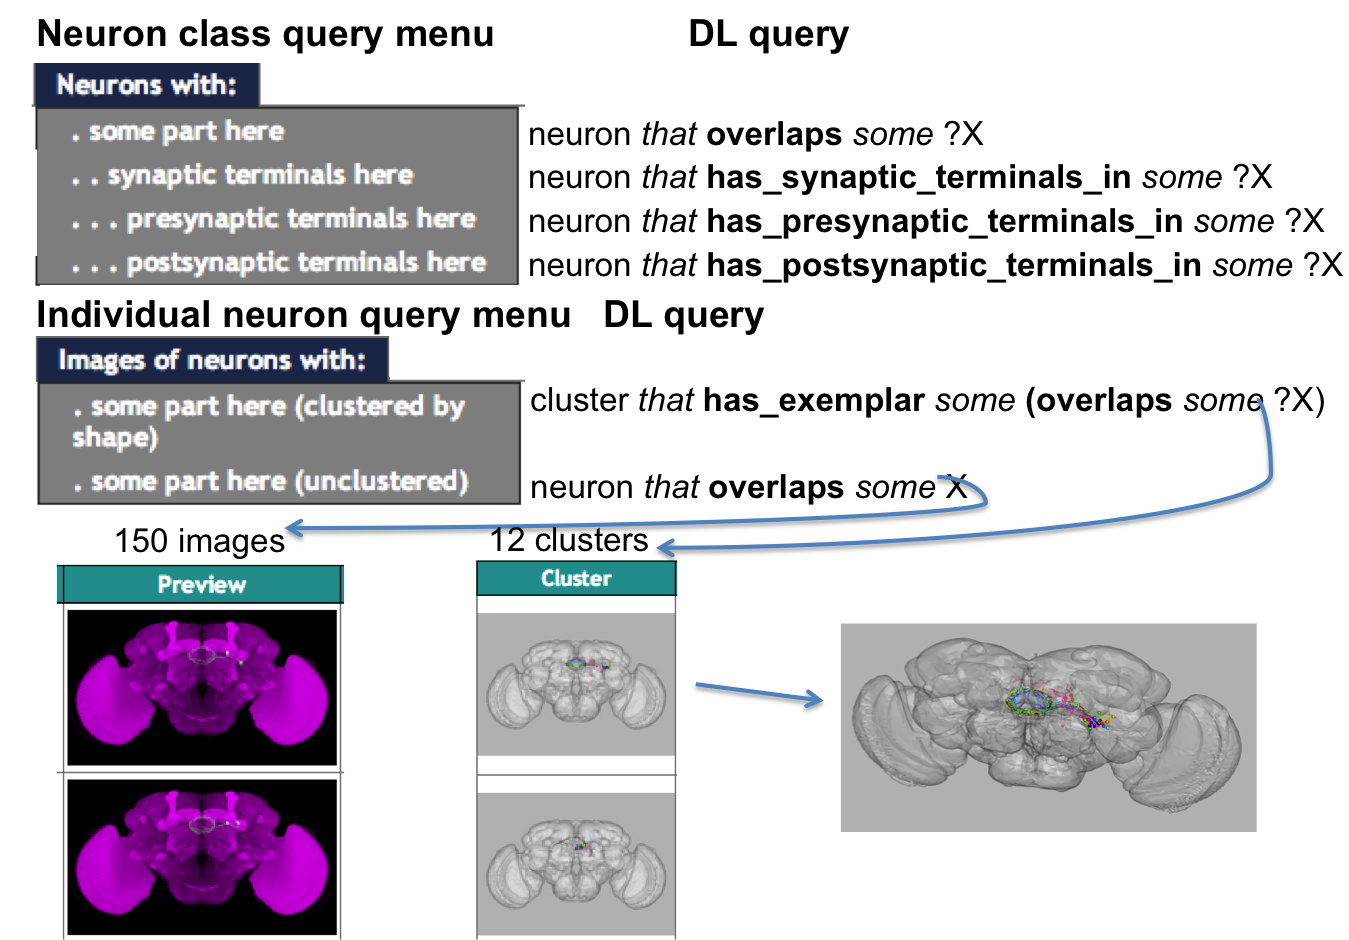
\includegraphics[width=120mm]{images/Query_menus_DL_images.png}
\caption{VFB query menus (left) with the DL queries they run (right).  The top panel
  shows nested queries for classes of neurons based on \textbf{overlaps} and its
  subproperties.  Each of these queries returns classes based on
  assertions further down the partonomy than the query term.  The
  bottom panel show queries for individual neurons with and without
  clustering.  A 3D cluster image is shown on the bottom right. }
\label{fig:Query_menus_DL_images}
\end{figure}

\section{Integration of images into VFB using OWL}

Neurobiology is a very visual subject.  While it is useful to read
both informal and formal descriptions of neuron classes and brain
regions, there is no substitute for being able to see images of them.
VFB is built around a standard, 3D adult brain image.  Major brain
regions are defined as 3D painted regions on this image according to
an expert-defined standard \cite{pmid24559671}.  These regions are modelled as
individual members of the relevant ontology classes, but are also
related to brain region classes via an axiom of the form:

\begin{quote}
\textbf{has\_exemplar} \textit{value} `individual region'
\end{quote}

This indicates that the individual provides a standard reference for
the boundaries of a brain region.  A simple DL query is used to find
images to illustrate term pages for these brain regions.

VFB also incorporates large datasets of 3D images of single neurons
(\textgreater 16,000), neuron clones (\textgreater 200) and expression
patterns (\textgreater 3500). As for painted brain regions, structures
depicted in these images are modelled as OWL individuals.
Importantly, all of these images are registered (morphed) onto the
standard brain. This allows direct comparison - both automated and
manual  - of registered images.

From image analysis, we can determine which gross brain regions a
neuron, clone or expression pattern \textbf{overlaps}, recording this
using a \textit{Type} statement on the individual.  These axioms drive queries for
single neuron images by location (figure
\ref{fig:Query_menus_DL_images}). A more sophisticated form of image
analysis, developed by G Jefferis [unpublished], compares pairs of
neurons,  giving each pair a similarity score based on morphology
and location.  A clustering algorithm is then used to group neurons with
similar morphology and location and to assign an exemplar neuron for
each cluster.

We treat clusters as individuals, with single neurons standing in a
\textbf{member\_of} relationship to a cluster.  A subproperty of
\textbf{member\_of}, \textbf{exemplar\_of}, is used to relate
exemplars to clusters.  This simple formalism allows VFB to group the
very large numbers of images that often result from queries of brain
regions for overlapping neurons into a much smaller number of clusters
of similar neurons (see figure \ref{fig:Query_menus_DL_images}).

In many cases, the resulting clusters correspond largely or completely
to well characterized neurons from the literature, for which the DAO
has classes defined by lineage, tract and location of synaptic
connections. Where this is the case, we add manual typing
statements. In other cases, manual annotation of neurons with
\textit{Type} statements provides sufficient information for automated
classification in the ontology.

\subsection{Modelling expression patterns in OWL}

A key aim of VFB is to provide a means for biologists to find
candidate transgenes suitable for use in genetic dissection of nervous
system function. This is aided immensely by providing images of the
expression patterns found.

To formalise what we mean by expression pattern, we first define a
relation, expresses:

\begin{quote}
\textbf{expresses}: This relation holds between an anatomical entity (a)
and a gene or transgene (g) where the anatomical entity is either a cell
or has cells as a part and in all of those cells, some instance of GO:gene
expression that has input g is occuring.
% Would be better if this were in common logic! But what is g? Might make sense if g
% was a GDC, but hard to explain that here.
\end{quote}


We use this relation to record expression in any type of cell or
multicellular anatomical entity including single neurons, neuron
clones and complete expression patterns.  Images of single neurons and
neuron clones typically depict only fragments of expression patterns.  To keep these
separable from images of complete expression patterns, we define an
expression pattern as an anatomical entity consisting of mereological
sum of all cells that express a particular gene or
transgene.  This is axiomatised using the following pattern:

\begin{quote}
`gene B expression pattern'
\textit{EquivalentTo}: `expression pattern' \textit{that} \textbf{expresses} \textit{some} `gene
B'\end{quote}
\begin{quote} \textit{GCI}: \textbf{expresses} \textbf{some} `gene B' \textit{EquivalentTo}
\textbf{part\_of} \textit{some} `B expression pattern'
\end{quote}


Classification time for the full ontology combined with the
knowledgebase (> 21,000 expression patterns, clones and neurons) is  ~
1500ms.  DL query answering time, taking advantage of incremental
reasoning with ELK, is under 100ms.

Representation of expression patterns in the knowledgebase is
currently used on VFB to provide images of transgene
expression patterns found via SQL queries. The above formalisation
provides an obvious way to convert the semi-formalised annotations in
SQL to OWL.

For brain regions:

\begin{quote}`expression pattern of X' \textbf{overlaps} \textit{some} `brain
region Y'  (see figure \ref{fig:exp_pat_neg} for an example)\end{quote}

For cells, we can make a stronger assertion:

\begin{quote}`expression pattern of X'
\textbf{has\_part}\footnote{\textbf{has\_part} entails \textbf{overlaps}} \textit{some} `cell Y' \end{quote}

We can then find anatomical structures in which there is some
expression via ``\textbf{overlaps} \textit{some} X''

As discussed in the next section, this formalisation can be used to as
part of a pattern that allows safe queries for expression patterns involving negation..

\section{Beyond EL: supporting queries with negation.}

In order to remain computationally tractable and scalable, VFB
restricts expressiveness to the EL profile of OWL and uses the ELK
reasoner \cite{kazakov2012elk} during development and to drive live
OWL queries on the site. Recent advances in reasoning
technology may make scaling with more expressive forms of OWL
practical. For example, Zhou and colleagues have recently published
impressive results for fast query answering by combining triple store
based RL reasoning with a HermiT DL reasoner \cite{ZNCH14a}.

Some types of queries that would be extremely useful to our users
require more expressiveness.  In particular, there are a number of
cases where queries involving negation would be useful.  For example,
for some neurons, we know all of the brain regions overlapped, all of
the tracts fasciculated with and the location of all synaptic
terminals.  It would be useful, in such cases, to allow users to add
negative legs to the compound queries for neuron classes that VFB
already supports.  For some transgene expression
patterns in the adult brain, we have both negative and positive
assertions about where a transgene is expressed.  It would be very
useful for researchers to be able to add negative clauses to queries for
expression as this can be critical for finding sufficiently
specific reagents to use to modulate the activity of specific neurons
to assess their function.

The most efficient way to support queries involving negation is to
combine closure axioms and disjointness declarations.  For
example, the neuron DL1 adPN fasciculates with only one tract, the
mALT.  We currently record this as:


\begin{quote}
`DL1 adPN' \textit{subClassOf} \textbf{fascicualtes\_with} \textit{some} mALT
\end{quote}

But if we also have the axioms:

\begin{quote}
`DL1 adPN' \textit{subClassOf} \textbf{fasciculates\_with} \textit{only} mALT

`great commissure' \textit{disjointWith} mALT
\end{quote}

Then we can find 'DL1 adPN' with the query:
\begin{quote}
	neuron \textit{and not} (\textbf{fasciculates\_with} \textit{some} `great commissure')
\end{quote}

For cases where a neuron \textbf{fasciculates\_with} multiple tracts, the
closure axioms can simply combine multiple classes using
\textit{or}. Unfortunately, our use of inference over partonomy rules out
this pattern of closure axioms for many important relations used in querying.  For example:

\begin{quote}
\textbf{overlaps} \textit{o} \textbf{part\_of} \textit{subPropertyOf}
\textbf{overlaps}

X \textbf{overlaps} \textit{some} Y

X \textbf{overlaps} \textit{only} Y

Y \textbf{part\_of} \textit{some} Z

Z \textit{disjointWith} X

=\textgreater inconsistency: X \textbf{overlaps} \textit{some} Z, X not (\textbf{overlaps}
\textit{some} Z)
\end{quote}


We can get around this by using closure axioms of the form
``\textbf{rel} \textit{only} (\textbf{has\_part} some X)'' and declaring spatial
disjointness between brain regions (which also provides a useful
integrity check). Spatial disjointness can be declared using a simple
GCI:

\begin{quote}
\textbf{part\_of} \textit{some} X \textit{disjointWith} \textbf{part\_of} \textit{some} Y
\end{quote}

For example, we can represent that the neuron DL1 adPN only has
synaptic terminals in DL1 (part of the antennal lobe) and the lateral
horn\footnote{There is  actually one additional region, but we
  simplify here in order to  provide a more compact example} with:

\begin{quote}
`DL1 adPN'

\textit{subClassOf}: \textbf{has\_synaptic\_terminals\_in}
\textit{some} DL1

\textit{subClassOf}: \textbf{has\_synaptic\_terminals\_in}
\textit{some} `lateral horn'

\textit{subClassOf}: \textbf{has\_synaptic\_terminals\_in}
\textit{only} (\textbf{has\_part} \textit{only} (DL1 \textit{or}
`lateral horn'))

`fan-shaped body' \textit{subClassOf}: \textbf{part\_of} \textit{some}
`central complex'

DL1 \textit{subClassOf}: \textbf{part\_of} \textit{some} `antennal lobe'
\end{quote}

With `antennal lobe', `lateral horn' and  `central complex' declared
spatially disjoint , DL1 adPN is returned by the query:

\begin{quote}
neuron that (\textbf{has\_synaptic\_terminal\_in} \textit{some}
`antennal lobe') and not (\textbf{has\_synaptic\_terminal\_in}
\textit{some} `fan-shaped body')
\end{quote}

An explanation is shown in figure \ref{fig:combined_explanation}B.  There is no need to
assert \textbf{has\_part} relationships. The
\textit{inverseOf} axiom between \textbf{has\_part} and
\textbf{part\_of} is sufficient to infer not \textbf{has\_part} from
spatial disjointness axioms (figure \ref{fig:combined_explanation}A).

This pattern is also dependent on the reflexive nature of
\textbf{part\_of} and \textbf{has\_part} (figure \ref{fig:combined_explanation}B).

\begin{figure}
\centering
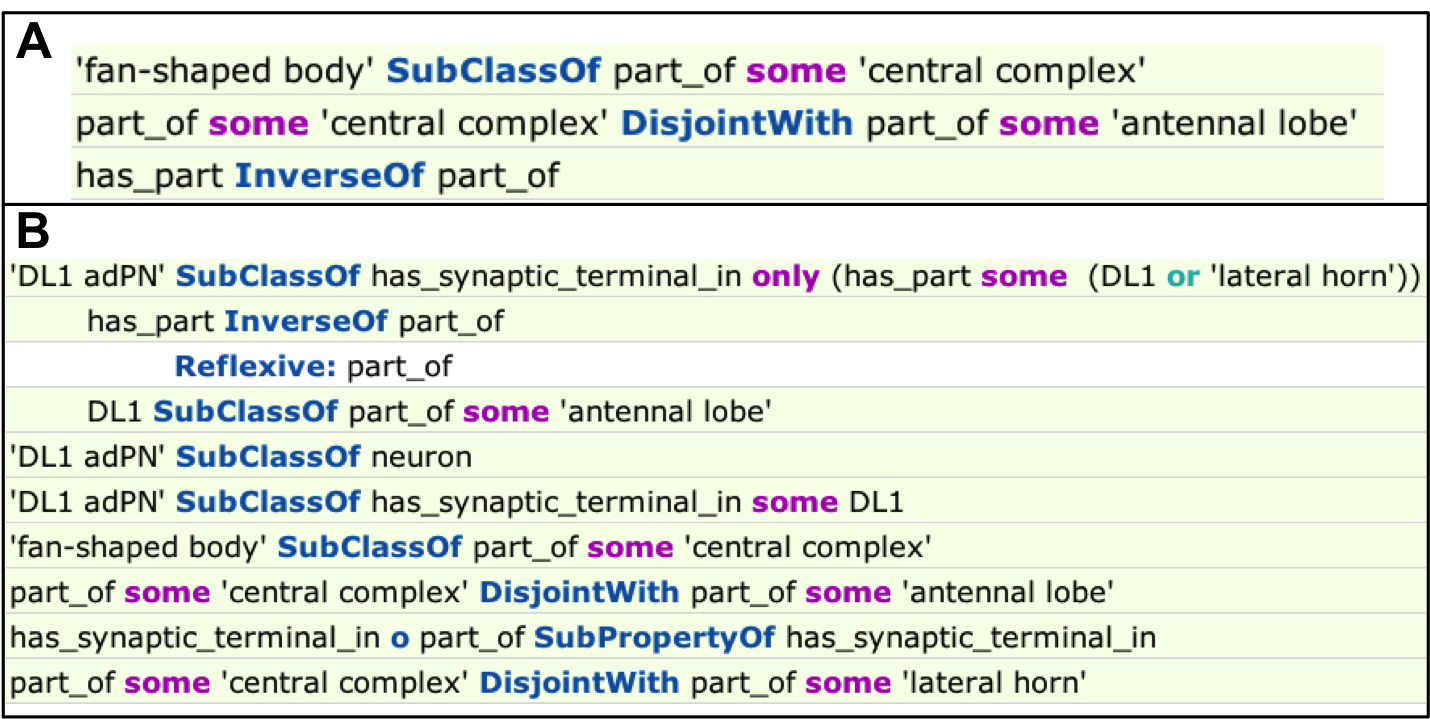
\includegraphics[width=120mm]{images/combined_explanation.png}
\caption{\textbf{A.} Explanation for why the query ``\textit{not}
   \textbf{has\_part} \textit{some} `fan-shaped body' '' returns
   `antennal lobe'.  Note that direct assertion of \textbf{has\_part}
   restriction axioms is not necessary. \textbf{B.} Explanation for
   why the query ``neuron that (\textbf{has\_synaptic\_terminal\_in}
   \textit{some} `antennal lobe') and not
   (\textbf{has\_synaptic\_terminal\_in} \textit{some} `fan-shaped
   body')'' returns the neuron `DL1 adPN'. }
\label{fig:combined_explanation}
\end{figure}

Negative query legs in compound queries for expression patterns would
be especially useful to our users.  Our ability to provide these is
limited by the extent to which it is possible to specify which regions
lack expression.  It is generally not possible to provide an
exhaustive list of all regions lacking
expression to use to define a closure axiom.  However some datasets
come with explicit assertions about regions not overlapped.  For
example, the largest transgene expression dataset that VFB currently
hosts \cite{pmid23063364} was provided with annotations recording the
presence or absence of expression in every major neuropil in the adult
brain.  These can easily be translated programmatically into restriction axioms
asserting \textbf{overlaps} and \textit{not} \textbf{overlaps} on
expression pattern classes (figure \ref{fig:exp_pat_neg}).

\begin{figure}
\centering
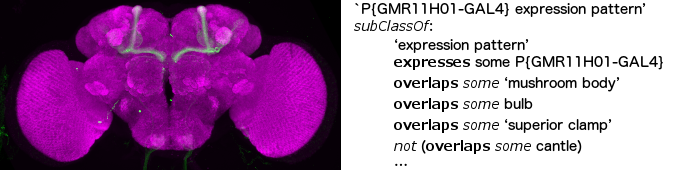
\includegraphics[width=120mm]{images/expression_pattern_with_neg.png}
\caption{The left panel shows the expression pattern of the
  P{GMR11H01-GAL4} transgene in the adult brain.  The right panel
  shows its representation in OWL. Only one explicit negation is shown,
  but the full OWL representation includes negative expression
  assertions for 30 brain regions.  These explicit negations are
  necessary in the absence of sufficient information to add closure axioms.}
\label{fig:exp_pat_neg}
\end{figure}

\section{Discussion and future directions}

% Section summarising VFBs work

Virtual Fly Brain uses OWL to provide a unique service to the
\textit{Drosophila} neurobiology community, integrating a wealth of
information from the literature and bulk datasets into an easily
queryable resource.  Much of this would be difficult or impossible to
provide using a conventional relational database. OWL
provides a sustainable way to develop and maintain a queryable
classification of anatomical structures and neurons.  OWL
axiomatisation allowing inference over partonomy drives queries that
 return complete information about neuronal overlap and synaptic
 terminal location from any level of the partonomy.  OWL reasoning
 also provides a way to group annotations of expression and phenotypes
 based on classification, partonomy and cell overlap.  This massively
 enriches the results of annotation queries.


VFB has so far avoided taking advantage of the full expressiveness of
OWL. Restricting expressiveness to the EL profile allows us to use the
ELK reasoner, which gives classification and query
answering times of < 500ms with our ontology and
knowledgeBase. Reasoners such as HermiT\cite{HermiT2008} and FaCT++
\cite{Fact2006}  are many orders of magnitude slower at classifying
the DAO and answering queries.  They do not even complete when
reasoning across the DAO combined with the VFB knowledgeBase of
individuals.  However, we have one use case for which DL
expressiveness would be extremely useful: compound queries for neurons
or expression patterns involving negation.

There are two major barriers to achieving this. The most serious
barrier is the ability to query across an ontology or combined ontology and
knowledgeBase with DL expressiveness.  Zhou and colleagues have
recently published impressive results for fast query answering by
combining triple store based RL reasoning with a HermiT DL reasoner
\cite{ZNCH14a}.  We are working with the authors to test query speed
for compound queries with negation for test datasets using the design
patterns outlined in this paper.

A more clearly surmountable barrier is the lack of tooling support for
some of the axiomatisation required in the design patterns we propose.  In
particular, adding GCIs to record spatial disjointness is currently
very tedious to do by hand in Protege 5.  This may be achievable by
scripting, but in order for the approach to be accessible for any
ontology builder this would ideally be achievable via a plugin for a
popular editor such as Protege.  By analogy with support for the
addition of class disjointness axioms in Protege, this could work by allowing
users to navigate down a partonomy tree, adding disjointness axioms to
whole sets of sibling terms at once.


\section{Methods}

For details of construction and maintenance of the \textit{Drosophila}
anatomy ontology please see Costa et al., 2013 \cite{Costa2013}. The
ontology is available from \url{http://purl.obolibrary.org/obo/fbbt}

VFB is an open source project.  All code is available from
\url{https://github.com/VirtualFlyBrain}
OWL individuals files used on VFB are available from
\url{https://github.com/VirtualFlyBrain/VFB_owl/tree/master/src/owl}. A
test ontology illustrating implementation of the DL patterns for
negative queries can be found at:
\url{https://github.com/VirtualFlyBrain/VFB_papers/owl/owled2014_demo.owl}

\subsection{VFB architecture}

All queries for anatomical classes or individuals on VFB are live DL
queries via the elk OWL reasoner.  All queries of annotation begin
with a DL query for subclasses, parts and overlapping cells.  The
resulting list is then used to query annotations store in the FlyBase
Postgresql database.  More details of the overall architecture of the
project cen be found at
\url{https://github.com/VirtualFlyBrain/VFB#overall-architecture-of-project}


\subsection{Database representation of OWL individuals}

Details of individuals are maintained in a SQL database
(\url{https://github.com/VirtualFlyBrain/VFB_owl/wiki/Individuals-DB})
and programmatically converted to OWL via scripting over the OWL-API
(\url{https://github.com/VirtualFlyBrain/VFB_owl/}).  A standard DB
representation of OWL ontologies/individuals would be preferable to
our bespoke solution, which limits axiom expressiveness in order to
keep the DB structure simple.  We are currently unaware of any viable,
non-proprietary alternatives.

\subsection*{Author's contributions}

The OWL design patterns and queries presented in this paper were designed and
tested by DOS  He also designed the database representation of OWL
individuals and wrote the code the translates this representation into
OWL. DOS, MC, and RC all contrubuted to the representation of
neuroanatomy in the  DAO.  MC  was also responsible for annotation of
individual neurons in the VFB knowldgeBase.

\subsection*{Acknowledgments.}

We thank all those who have contributed to the development of VFB who
are not authors on this paper: FlyBase, Michael Ashburner, J. Douglas
Armstrong, Nestor Milyaev, Simon Reeve and Gregory S.X.E Jefferis.

\subsubsection*{Funding}

This work was largely supported by:`Standardising the representation of
Drosophila anatomy and development for databases' 
BBBSRC:BB/G02233X/1 awarded 2009 to J.Douglas Armstrong, Michael 
Ashburner, Cahir O'Kane and David Osumi-Sutherland;  An Isaac Newton
Trust grant to Cahir O'Kane to fund the work of Marta Costa, Awarded
2012:`Neuroinformatic identification of new types of neuron in the
Drosophila brain.' VFB is currently supported by a Wellcome Trust
grant to Cahir O'Kane, J. Douglas Armstrong, Gregory S.X.E Jefferis,
Helen Parkinson and David Osumi-Sutherland: `Virtual Fly Brain: a
global informatics hub for Drosophila neurobiology' WT105023MA.

%\begin{thebibliography}{}

\bibliography{owled2014} % Bibliography file (usually '*.bib' )

\bibliographystyle{plain}

%\end{thebibliography}

\end{document}
